\ifx\wholebook\relax \else
% ------------------------ 

\documentclass{article}
%------------------- Other types of document example ------------------------
%
%\documentclass[twocolumn]{IEEEtran-new}
%\documentclass[12pt,twoside,draft]{IEEEtran}
%\documentstyle[9pt,twocolumn,technote,twoside]{IEEEtran}
%
%-----------------------------------------------------------------------------
%%
% loading packages
%
\newif\ifpdf
\ifx\pdfoutput\undefined % We're not running pdftex
  \pdffalse
\else
  \pdftrue
\fi
%
%
\ifpdf
  \RequirePackage[pdftex,%
            CJKbookmarks,%
       bookmarksnumbered,%
              colorlinks,%
          linkcolor=blue,%
              hyperindex,%
        plainpages=false,%
       pdfstartview=FitH]{hyperref}
\else
  \RequirePackage[dvipdfm,%
             CJKbookmarks,%
        bookmarksnumbered,%
               colorlinks,%
           linkcolor=blue,%
               hyperindex,%
         plainpages=false,%
        pdfstartview=FitH]{hyperref}
  \AtBeginDvi{\special{pdf:tounicode GBK-EUC-UCS2}} % GBK -> Unicode
\fi
\usepackage{hyperref}

% other packages
%-----------------------------------------------------------------------------
\usepackage{graphicx, color}
\usepackage{CJK}
%
% for programming 
%
\usepackage{verbatim}
\usepackage{listings}


\lstdefinelanguage{Smalltalk}{
  morekeywords={self,super,true,false,nil,thisContext}, % This is overkill
  morestring=[d]',
  morecomment=[s]{"}{"},
  alsoletter={\#:},
  escapechar={!},
  literate=
    {BANG}{!}1
    {UNDERSCORE}{\_}1
    {\\st}{Smalltalk}9 % convenience -- in case \st occurs in code
    % {'}{{\textquotesingle}}1 % replaced by upquote=true in \lstset
    {_}{{$\leftarrow$}}1
    {>>>}{{\sep}}1
    {^}{{$\uparrow$}}1
    {~}{{$\sim$}}1
    {-}{{\sf -\hspace{-0.13em}-}}1  % the goal is to make - the same width as +
    %{+}{\raisebox{0.08ex}{+}}1		% and to raise + off the baseline to match -
    {-->}{{\quad$\longrightarrow$\quad}}3
	, % Don't forget the comma at the end!
  tabsize=2
}[keywords,comments,strings]

\lstloadlanguages{C++, Lisp, Haskell, Python, Smalltalk}

% ======================================================================

\def\BibTeX{{\rm B\kern-.05em{\sc i\kern-.025em b}\kern-.08em
    T\kern-.1667em\lower.7ex\hbox{E}\kern-.125emX}}

\newtheorem{theorem}{Theorem}

%
% mathematics
%
\newcommand{\be}{\begin{equation}}
\newcommand{\ee}{\end{equation}}
\newcommand{\bmat}[1]{\left( \begin{array}{#1} }
\newcommand{\emat}{\end{array} \right) }
\newcommand{\VEC}[1]{\mbox{\boldmath $#1$}}

% numbered equation array
\newcommand{\bea}{\begin{eqnarray}}
\newcommand{\eea}{\end{eqnarray}}

% equation array not numbered
\newcommand{\bean}{\begin{eqnarray*}}
\newcommand{\eean}{\end{eqnarray*}}

\RequirePackage{CJK,CJKnumb,CJKulem,CJKpunct}
% we use CJK as default environment
\AtBeginDocument{\begin{CJK*}{GBK}{song}\CJKtilde\CJKindent\CJKcaption{GB}}
\AtEndDocument{\clearpage\end{CJK*}}

%
% loading packages
%

\RequirePackage{ifpdf}

%
%
\ifpdf
  \RequirePackage[pdftex,%
       bookmarksnumbered,%
              colorlinks,%
          linkcolor=blue,%
              hyperindex,%
        plainpages=false,%
       pdfstartview=FitH]{hyperref}
\else
  \RequirePackage[dvipdfm,%
        bookmarksnumbered,%
               colorlinks,%
           linkcolor=blue,%
               hyperindex,%
         plainpages=false,%
        pdfstartview=FitH]{hyperref}
\fi
\usepackage{hyperref}

% other packages
%--------------------------------------------------------------------------
\usepackage{graphicx, color}
\usepackage{subfig}

\usepackage{amsmath, amsthm, amssymb} % for math
\usepackage{exercise} % for exercise

%
% for programming 
%
\usepackage{verbatim}
\usepackage{listings}
%\usepackage{algorithmic} %old version; we can use algorithmicx instead
\usepackage{algorithm} 
\usepackage[noend]{algpseudocode} %for pseudo code, include algorithmicsx automatically
\usepackage{makeidx} % for index support


\lstdefinelanguage{Smalltalk}{
  morekeywords={self,super,true,false,nil,thisContext}, % This is overkill
  morestring=[d]',
  morecomment=[s]{"}{"},
  alsoletter={\#:},
  escapechar={!},
  literate=
    {BANG}{!}1
    {UNDERSCORE}{\_}1
    {\\st}{Smalltalk}9 % convenience -- in case \st occurs in code
    % {'}{{\textquotesingle}}1 % replaced by upquote=true in \lstset
    {_}{{$\leftarrow$}}1
    {>>>}{{\sep}}1
    {^}{{$\uparrow$}}1
    {~}{{$\sim$}}1
    {-}{{\sf -\hspace{-0.13em}-}}1  % the goal is to make - the same width as +
    %{+}{\raisebox{0.08ex}{+}}1		% and to raise + off the baseline to match -
    {-->}{{\quad$\longrightarrow$\quad}}3
	, % Don't forget the comma at the end!
  tabsize=2
}[keywords,comments,strings]

\lstloadlanguages{C++, Lisp, Haskell, Python, Smalltalk}

% ======================================================================

\def\BibTeX{{\rm B\kern-.05em{\sc i\kern-.025em b}\kern-.08em
    T\kern-.1667em\lower.7ex\hbox{E}\kern-.125emX}}

%
% mathematics
%
\newcommand{\be}{\begin{equation}}
\newcommand{\ee}{\end{equation}}
\newcommand{\bmat}[1]{\left( \begin{array}{#1} }
\newcommand{\emat}{\end{array} \right) }
\newcommand{\VEC}[1]{\mbox{\boldmath $#1$}}

% numbered equation array
\newcommand{\bea}{\begin{eqnarray}}
\newcommand{\eea}{\end{eqnarray}}

% equation array not numbered
\newcommand{\bean}{\begin{eqnarray*}}
\newcommand{\eean}{\end{eqnarray*}}

\newtheorem{theorem}{Theorem}[section]
\newtheorem{lemma}[theorem]{Lemma}
\newtheorem{proposition}[theorem]{Proposition}
\newtheorem{corollary}[theorem]{Corollary}


\setcounter{page}{1}

\begin{document}

\fi
%--------------------------

% ================================================================
%                 COVER PAGE
% ================================================================

\title{The evolution of insertion sort}

\author{Liu~Xinyu
\thanks{{\bfseries Liu Xinyu } \newline
  Email: liuxinyu95@gmail.com \newline}
  }

\markboth{The evolution of insertion sort}{AlgoXY}

\maketitle

\ifx\wholebook\relax
\chapter{The evolution of insertion sort}
\numberwithin{Exercise}{chapter}
\fi

% ================================================================
%                 Introduction
% ================================================================
\section{Introduction}
\label{introduction} \index{insertion sort}
In previous chapter, we introduced the 'hello world' data structure,
binary search tree. In this chapter, we explain insertion sort,
which can be think of the 'hello world' sorting algorithm 
\footnote{Some reader may argue that 'Bubble sort' is the easiest
sort algorithm. Bubble sort isn't covered in this book as we don't
think it's a valuabel algorithm\cite{wiki-bubble-sort}}.
It's straightforward, but the performance is not as good as some
divide and conqueror sorting approaches, such as quick sort
and merge sort. Thus insertion sort is seldom used as generic
sorting utility in modern software libraries. We'll analyze the 
problems why it is slow, and trying to improve it bit by bit till
we reach the best bound of comparison based sorting algorithms, $O(N \lg N)$,
by evoluting to tree sort. And we finally show the connection between
the 'hello world' data structure and 'hello world' sorting algorithm. 

The idea of insertion sort can be vivid illustrated by a real life
poker game\cite{CLRS}. Suppose the cards are shuffled, and a player starts 
taking card one by one.

At any time, all cards in player's hand are well sorted. When the player
gets a new card, he insert it in proper position according to the order
of points. Figure \ref{fig:hand-of-cards} shows this insertion example.

\begin{figure}[htbp]
  \centering
  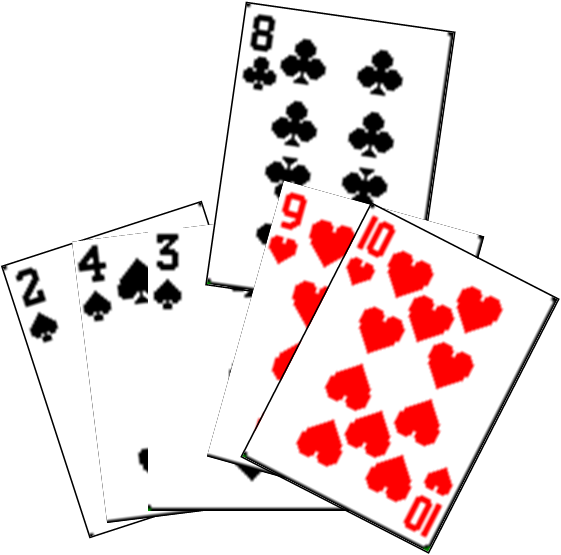
\includegraphics[scale=0.5]{img/hand-of-cards.eps}
  \caption{Insert card 8 to proper position in a deck.} 
  \label{fig:hand-of-cards}
\end{figure}

Based on this idea, the algorithm of insertion sort can be directly
given as the following.

\begin{algorithmic}
\Function{Sort}{$A$}
  \State $X \gets \Phi$
  \For{each $x \in A$}
    \State \Call{Insert}{$X, x$}
  \EndFor
  \State \Return $X$
\EndFunction
\end{algorithmic}

It's easy to express this process with folding, which we 
mentioned in the chapter of binary search tree.

\be
  insert = foldL \quad insert \quad \Phi
\ee

Note that in above algorithm, we store the sorted result in $X$, 
so this isn't in-place sorting. It's easy to change it to in-plance
algorithm.

\begin{algorithmic}
\Function{Sort}{$A$}
  \For{$i \gets 2$ to \Call{Length}{$A$}}
    \State insert $A_i$ to sorted sequence $\{A'_1, A'_2, ..., A'_{i-1} \}$
  \EndFor
\EndFunction
\end{algorithmic}

TODO: add figure to illustrate the idea

We can find there are recursive concept in this definition. Thus it can
be expressed as the following.

\be
sort(A) = \left \{
  \begin{array}
  {r@{\quad:\quad}l}
  \Phi & A = \Phi \\
  insert(sort(\{A_2, A_3, ...\}), A_1) & otherwise
  \end{array}
\right.  
\ee

% ================================================================
% Insertion
% ================================================================
\section{Insertion}
\index{insertion sort!insertion}

We haven't answered the question about how to realize insertion however.
It's a puzzle how does human locate the proper postion so quickly?

For computer, it's an obvious option to perform a scan. We can either 
scan from left to right or vice versa. However, if the sequence is
stored in plain array, it's neccessary to scan from right to left.

TODO: Add algorithm

One may think scan from left to right is natural. However, 

% ================================================================
% Insert
% ================================================================
\section{Insertion}
\index{binary search tree!insertion}

To insert a key $k$ (may be along with a value in practice) to a binary search tree $T$, we can follow a quite straight forward way.

\begin{itemize}
\item If the tree is empty, then construct a leave node with key=$k$;
\item If $k$ is less than the key of root node, insert it to the left child;
\item If $k$ is greater than the key of root, insert it to the right child;
\end{itemize}

There is an exceptional case that if $k$ is equal to the key of root, it means it has already existed, we can either overwrite the data, or just do nothing.
For simple reason, this case is skipped in this post.

This algorithm is described recursively. It is so simple that is why we 
consider binary search tree is `hello world' data structure. Formally, 
the algorithm can be represented with a recursive function.

\be
insert(T, k) = \left \{
  \begin{array}
  {r@{\quad:\quad}l}
  node(\phi, k, \phi) & T = \phi \\
  node(insert(L, k), Key, R) & k < Key \\
  node(L, Key, insert(R, k)) & otherwise
  \end{array}
\right.
\ee 

Where 
\[
  \begin{array}{l}
  L = left(T) \\
  R = right(T) \\
  Key = key(T)
  \end{array}
\]

The node function creates a new node with given left sub-tree,
a key and a right sub-tree as parameters. $\phi$ means NIL or Empty.
function $left$, $right$ and $key$ are access functions which can 
get the left sub-tree, right sub-tree and the key of a node.

Translate the above functions directly to Haskell yields the following
program.

\lstset{language=Haskell}
\begin{lstlisting}
insert::(Ord a) => Tree a -> a -> Tree a
insert Empty k = Node Empty k Empty
insert (Node l x r) k | k < x = Node (insert l k) x r
                      | otherwise = Node l x (insert r k)
\end{lstlisting}

This program utilized the pattern matching features provided by the 
language. However, even in functional settings without this feature,
for instance, Scheme/Lisp, the program is still expressive.

\lstset{language=lisp}
\begin{lstlisting}
(define (insert tree x)
  (cond ((null? tree) (list '() x '()))
	((< x (key tree))
	 (make-tree (insert (left tree) x)
		    (key tree)
		    (right tree)))
	((> x (key tree))
	 (make-tree (left tree)
		    (key tree)
		    (insert (right tree) x)))))
\end{lstlisting}

It is possible to turn the algorithm completely into imperative way
without recursion. 

\begin{algorithmic}[1]
\Function{Insert}{$T, k$}
  \State $root \gets T$
  \State $x \gets$ \Call{Create-Leaf}{$k$}
  \State $parent \gets NIL$
  \While{$T \neq NIL$}
    \State $parent \gets T$
    \If{$k <$ \Call{Key}{$T$}}
      \State $T \gets $ \Call{Left}{$T$}
    \Else
      \State $T \gets $ \Call{Right}{$T$}
    \EndIf
  \EndWhile
  \State \Call{Parent}{$x$} $\gets parent$
  \If{$parent = NIL$} \Comment{tree $T$ is empty}
    \State \Return $x$
  \ElsIf{$k <$ \Call{Key}{$parent$}}
    \State \Call{Left}{$parent$} $\gets x$
  \Else
    \State \Call{Right}{$parent$} $\gets x$
  \EndIf
  \State \Return $root$
\EndFunction
\Statex
\Function{Create-Leaf}{k}
  \State $x \gets $ \Call{Empty-Node}{}
  \State \Call{Key}{$x$} $ \gets k$
  \State \Call{Left}{$x$} $ \gets NIL$
  \State \Call{Right}{$x$} $ \gets NIL$
  \State \Call{Parent}{$x$} $ \gets NIL$
  \State \Return $x$
\EndFunction
\end{algorithmic}

Compare with the functional algorithm, it is obviously that this one
is more complex although it is fast and can handle very deep tree. A 
complete C++ program and a python program are available along with this
post for reference.

\section{Traversing}
\index{binary search tree!traverse}

Traversing means visiting every element one by one in a binary 
search tree. There are 3 ways to traverse a binary tree, pre-order tree walk, 
in-order tree walk, and post-order tree walk. The names of these
traversing methods highlight the order of when we visit the root
of a binary search tree.

Since there are three parts in a tree, as left child, the root, which
contains the key and satellite data, and the right child. If we denote
them as $(left, current, right)$, the three traversing methods are defined 
as the following.

\begin{itemize}
\item pre-order traverse, visit $current$, then $left$, finally $right$;
\item in-order traverse, visit $left$ , then $current$, finally $right$;
\item post-order traverse, visit $left$, then $right$, finally $current$.
\end{itemize}

\index{pre-order traverse} \index{in-order traverse} \index{post-order traverse}

Note that each visiting operation is recursive. And we see the order
of visiting $current$ determines the name of the traversing method.

For the binary search tree shown in figure \ref{fig:bst-example}, below
are the three different traversing results.

\begin{itemize}
\item pre-order traverse result: 4, 3, 1, 2, 8, 7, 16, 10, 9, 14;
\item in-order traverse result: 1, 2, 3, 4, 7, 8, 9, 10, 14, 16;
\item post-order traverse result: 2, 1, 3, 7, 9, 14, 10, 16, 8, 4;
\end{itemize}

It can be found that the in-order walk of a binary search tree outputs
the elements in increase order, which is particularly helpful. The definition
of binary search tree ensures this interesting property, while the
proof of this fact is left as an exercise of this post.

In-order tree walk algorithm can be described as the following:
\begin{itemize}
\item If the tree is empty, just return;
\item traverse the left child by in-order walk, then access the key, 
finally traverse the right child by in-order walk.
\end{itemize}

Translate the above description yields a generic map function

\be
map(f, T) = \left \{
  \begin{array}
  {r@{\quad:\quad}l}
  \phi & T = \phi \\
  node(l', k', r') & otherwise
  \end{array}
\right .
\ee

where

\[
 \begin{array}{l}
 l' = map(f, left(T)) \\
 r' = map(f, right(T)) \\
 k' = f(key(T))
 \end{array}
\]

If we only need access the key without create the transformed tree,
we can realize this algorithm in procedural way lie the below C++
program.

\lstset{language=C++}
\begin{lstlisting}
template<class T, class F>
void in_order_walk(node<T>* t, F f){
  if(t){
    in_order_walk(t->left, f);
    f(t->value);
    in_order_walk(t->right, f);
  }
}
\end{lstlisting}

The function takes a parameter f, it can be a real function, or a function
object, this program will apply f to the node by in-order tree walk.

We can simplified this algorithm one more step to define a function 
which turns a binary search tree to a sorted list by in-order traversing.

\be
toList(T) = \left \{
  \begin{array}
  {r@{\quad:\quad}l}
  \phi & T = \phi \\
  toList(left(T)) \cup \{ key(T) \} \cup toList(right(T)) & otherwise
  \end{array}
\right .
\ee

Below is the Haskell program based on this definition.

\lstset{language=Haskell}
\begin{lstlisting}
toList::(Ord a)=>Tree a -> [a]
toList Empty = []
toList (Node l x r) = toList l ++ [x] ++ toList r
\end{lstlisting}

This provides us a method to sort a list of elements. We can first
build a binary search tree from the list, then output the tree
by in-order traversing. This method is called as `tree sort'.
Let's denote the list $X = \{x_1, x_2, x_3, ..., x_n\}$.

\be
  sort(X) = toList(fromList(X))
\ee

And we can write it in function composition form.

\[
  sort = toList . fromList
\]

Where function $fromList$ repeatedly insert every element to a 
binary search tree.

\be
  fromList(X)= foldL(insert, \phi, X)
\ee

It can also be written in partial application form like below.

\[
  fromList = foldL \quad insert \quad \phi
\]

For the readers who are not familiar with folding from left, this function
can also be defined recursively as the following.

\[
fromList(X) = \left \{
  \begin{array}
  {r@{\quad:\quad}l}
  \phi & X = \phi \\
  insert(fromList(\{x_2, x_3, ..., x_n\}), x_1) & otherwise
  \end{array}
\right .
\]

We'll intense use folding function as well as the function composition
and partial evaluation in the future, please refer to \cite{wiki-fold}
\cite{func-composition} and \cite{curry} for more information.

\begin{Exercise}

\begin{itemize}
\item Given the in-order traverse result and pre-order traverse result, 
can you re-construct the tree from these result and figure out the 
post-order traversing result?

Pre-order result: 1, 2, 4, 3, 5, 6;
In-order result: 4, 2, 1, 5, 3, 6;
Post-order result: ?
\index{tree reconstruction}

\item Write a program in your favorite language to re-construct
the binary tree from pre-order result and in-order result.

\item Prove why in-order walk output the elements stored in a binary
search tree in increase order?

\item Can you analyze the performance of tree sort with big-O notation?
\end{itemize}
\end{Exercise}

% ================================================================
% Querying a binary search tree
% ================================================================
\section{Querying a binary search tree}
\index{binary search tree!search}
\index{binary search tree!looking up}

There are three types of querying for binary search tree, searching
a key in the tree, find the minimum or maximum element in the tree,
and find the predecessor or successor of an element in the tree.

\subsection{Looking up}
According to the definition of binary search tree, search
a key in a tree can be realized as the following.

\begin{itemize}
\item If the tree is empty, the searching fails;
\item If the key of the root is equal to the value to be found, the
search succeed. The root is returned as the result;
\item If the value is less than the key of the root, search in the left
child.
\item Else, which means that the value is greater than the key of the 
root, search in the right child.
\end{itemize}

This algorithm can be described with a recursive function as below.

\be
lookup(T, x) = \left \{
  \begin{array}
  {r@{\quad:\quad}l}
  \phi & T = \phi \\
  T & key(T) = x \\
  lookup(left(T), x) & x < key(T) \\
  lookup(right(T), x) & otherwise
  \end{array}
\right .
\ee

In the real application, we may return the satellite data instead of the
node as the search result. This algorithm is simple and straightforward.
Here is a translation of Haskell program.

\lstset{language=Haskell}
\begin{lstlisting}
lookup::(Ord a)=> Tree a -> a -> Tree a
lookup Empty _ = Empty
lookup t@(Node l k r) x | k == x = t
                        | x < k = lookup l x
                        | otherwise = lookup r x
\end{lstlisting}

If the binary search tree is well balanced, which means that almost
all nodes have both non-NIL left child and right child, for $N$ elements,
the search algorithm takes $O(\lg N)$ time to perform. This is not
formal definition of balance. We'll show it in later post about red-black-tree.
If the tree is poor balanced, the worst case takes $O(N)$ time to 
search for a key. If we denote the height of the tree as $h$, we can
uniform the performance of the algorithm as $O(h)$.

The search algorithm can also be realized without using recursion in 
a procedural manner.

\begin{algorithmic}[1]
\Function{Search}{$T, x$}
  \While{$T \neq NIL \wedge$ \Call{Key}{$T$} $ \neq x$}
    \If{$x <$ \Call{Key}{$T$}}
      \State $T \gets $ \Call{Left}{$T$}
    \Else
      \State $T \gets $ \Call{Right}{$T$}
    \EndIf
  \EndWhile
  \State \Return $T$
\EndFunction
\end{algorithmic}

Below is the C++ program based on this algorithm.

\lstset{language=C++}
\begin{lstlisting}
template<class T>
node<T>* search(node<T>* t, T x){
  while(t && t->key!=x){
    if(x < t->key) t=t->left;
    else t=t->right;
  }
  return t;
}
\end{lstlisting}

\subsection{Minimum and maximum}
\index{binary search tree!min/max}

Minimum and maximum can be implemented from the property of binary search
tree, less keys are always in left child, and greater keys are in right.

For minimum, we can continue traverse the left sub tree until it is empty.
While for maximum, we traverse the right.

\be
min(T) = \left \{
  \begin{array}
  {r@{\quad:\quad}l}
  key(T) & left(T) = \phi \\
  min(left(T)) & otherwise
  \end{array}
\right .
\ee

\be
max(T) = \left \{
  \begin{array}
  {r@{\quad:\quad}l}
  key(T) & right(T) = \phi \\
  max(right(T)) & otherwise
  \end{array}
\right .
\ee

Both function bound to $O(h)$ time, where $h$ is the height of the tree.
For the balanced binary search tree, $min$/$max$ are bound to $O(\lg N)$ time,
while they are $O(N)$ in the worst cases.

We skip translating them to programs, It's also possible to implement them 
in pure procedural way without using recursion.

\subsection{Successor and predecessor}
\index{binary search tree!succ/pred}

The last kind of querying, to find the successor or predecessor of an element
is useful when a tree is treated as a generic container and traversed by 
using iterator. It will be relative easier to implement if parent of
a node can be accessed directly. 

It seems that the functional solution is hard to be found, because there
is no pointer like field linking to the parent node. However, If we consider
the original purpose of providing $succ$/$pred$ function, `to traverse all the
binary search tree elements one by one` as a generic container, we realize
that they don't make significant sense in functional settings because 
we can traverse the tree in increase order by $mapT$ function we defined 
previously.

We'll meet many problems in this series of post that they are only valid
in imperative settings, and they are not meaningful problems in functional
settings at all. One good example is how to delete an element in 
red-black-tree\cite{okasaki-blog}.

In this section, we'll only present the imperative algorithm for finding
the successor and predecessor in a binary search tree.

When finding the successor of element $x$, which is the smallest one $y$
that satisfies $y > x$, there are two cases. If the node with value $x$
has non-NIL right child, the minimum element in right child is the answer;
For example, in Figure \ref{fig:bst-example}, in order to find the successor
of 8, we search it's right sub tree for the minimum one, which yields 9
as the result. While if node $x$ don't have right child, we need 
back-track to find the closest ancestors whose left child is also ancestor
of $x$. In Figure \ref{fig:bst-example}, since 2 don't have right sub tree,
we go back to its parent 1. However, node 1 don't have left child, so we
go back again and reach to node 3, the left child of 3, is also ancestor
of 2, thus, 3 is the successor of node 2.

Based on this description, the algorithm can be given as the following.

\begin{algorithmic}[1]
\Function{Succ}{$x$}
  \If{\Call{Right}{$x$} $\neq NIL$}
    \State \Return \textproc{Min}(\Call{Right}{$x$})
  \Else
    \State $p \gets $ \Call{Parent}{$x$}
    \While{$p \neq NIL$ and $x =$ \Call{Right}{$p$}}
      \State $x \gets p$
      \State $p \gets $ \Call{Parent}{$p$}
    \EndWhile
    \State \Return $p$
  \EndIf
\EndFunction
\end{algorithmic}

The predecessor case is quite similar to the successor algorithm, they
are symmetrical to each other. 

\begin{algorithmic}[1]
\Function{Pred}{$x$}
  \If{\Call{Left}{$x$} $\neq NIL$}
    \State \Return \textproc{Max}(\Call{Left}{$x$})
  \Else
    \State $p \gets $ \Call{Parent}{$x$}
    \While{$p \neq NIL$ and $x =$ \Call{Left}{$p$}}
      \State $x \gets p$
      \State $p \gets $ \Call{Parent}{$p$}
    \EndWhile
    \State \Return $p$
  \EndIf
\EndFunction
\end{algorithmic}

Below are the Python programs based on these algorithms. They are changed
a bit in while loop conditions.

\lstset{language=Python}
\begin{lstlisting}
def succ(x):
    if x.right is not None: return tree_min(x.right)
    p = x.parent
    while p is not None and p.left != x:
        x = p
        p = p.parent
    return p

def pred(x):
    if x.left is not None: return tree_max(x.left)
    p = x.parent
    while p is not None and p.right != x:
        x = p
        p = p.parent
    return p
\end{lstlisting}

\begin{Exercise}

\begin{itemize}
\item Can you figure out how to iterate a tree as a generic container
by using $pred()$/$succ()$? What's the performance of such traversing
process in terms of big-O?

\item A reader discussed about traversing all elements inside a 
range $[a, b]$. In C++, the algorithm looks like the below code:

$\mathbf{for\_each} (m.lower\_bound(12), m.upper\_bound(26), f);$

Can you provide the purely function solution for this problem?
\index{range traverse}
\end{itemize}

\end{Exercise}

% ================================================================
%                 Deletion
% ================================================================
\section{Deletion}
\index{binary search tree!delete}
Deletion is another `imperative only' topic for binary search tree.
This is because deletion mutate the tree, while in purely functional
settings, we don't modify the tree after building it in most 
application.

However, One method of deleting element from binary search
tree in purely functional way is shown in this section. It's actually
reconstructing the tree but not modifying the tree.

Deletion is the most complex operation for binary search tree. 
this is because we must keep the BST property, that for any node,
all keys in left sub tree are less than the key of this node, and
they are all less than any keys in right sub tree. Deleting a node
can break this property.

In this post, different with the algorithm described in \cite{CLRS}, 
A simpler one from SGI STL implementation is used.\cite{sgi-stl}

To delete a node $x$ from a tree.
\begin{itemize}
\item If $x$ has no child or only one child, splice x out;
\item Otherwise ($x$ has two children), use minimum element of its right sub tree to replace $x$, and splice the original minimum element out.
\end{itemize}

The simplicity comes from the truth that, the minimum element is stored
in a node in the right sub tree, which can't have two non-NIL children.
It ends up in the trivial case, the the node can be directly splice
out from the tree.

Figure \ref{fig:del-leaf}, \ref{fig:del-1child}, and \ref{fig:del-branch}
illustrate these different cases when deleting a node from the tree.

Based on this idea, the deletion can be defined as the below function.

\be
delete(T, x) = \left \{
  \begin{array}
  {r@{\quad:\quad}l}
  \phi & T = \phi \\
  node(delete(L, x), K, R) & x < K \\
  node(L, K, delete(R, x)) & x > K \\
  R & x = K \wedge L = \phi \\
  L & x = K \wedge R = \phi \\
  node(L, y, delete(R, y)) & otherwise
  \end{array}
\right .
\ee

Where
\[
\begin{array}{l}
L = left(T) \\
R = right(T) \\
K = key(T) \\
y = min(R)
\end{array}
\]

Translating the function to Haskell yields the below program.

\lstset{language=Haskell}
\begin{lstlisting}
delete::(Ord a)=> Tree a -> a -> Tree a
delete Empty _ = Empty
delete (Node l k r) x | x < k = (Node (delete l x) k r)
                      | x > k = (Node l k (delete r x))
                      -- x == k
                      | isEmpty l = r
                      | isEmpty r = l
                      | otherwise = (Node l k' (delete r k')) 
                          where k' = min r
\end{lstlisting}

Function `isEmpty' is used to test if a tree is empty ($\phi$).
Note that the algorithm first performs search to locate the node
where the element need be deleted, after that it execute the 
deletion. This algorithm takes $O(h)$ time where $h$ is the height
of the tree.

It's also possible to pass the node but not the element to the 
algorithm for deletion. Thus the searching is no more needed.

The imperative algorithm is more complex because it need set the 
parent properly. The function will return the root of the result tree.

\begin{algorithmic}[1]
\Function{Delete}{$T, x$}
  \State $root \gets T$
  \State $x' \gets x$ \Comment{save $x$}
  \State $parent \gets $ \Call{Parent}{$x$}
  \If{\Call{Left}{$x$} $= NIL$}
    \State $x \gets $ \Call{Right}{$x$}
  \ElsIf{\Call{Right}{$x$} $= NIL$}
    \State $x \gets $ \Call{Left}{$x$}
  \Else
    \Comment{both children are non-NIL}
    \State  $y \gets $ \textproc{Min}(\Call{Right}{$x$})
    \State \Call{Key}{$x$} $\gets$ \Call{Key}{$y$}
    \State Copy other satellite data from $y$ to $x$
    \If{\Call{Parent}{$y$} $\neq x$}
      \Comment{$y$ hasn't left sub tree}
      \State \textproc{Left}(\Call{Parent}{$y$}) $\gets$ \Call{Right}{$y$}
    \Else
      \Comment{$y$ is the root of right child of $x$}
      \State \Call{Right}{$x$} $\gets$ \Call{Right}{$y$}
    \EndIf
    \State Remove $y$
    \State \Return $root$
  \EndIf
  \If{$x \neq NIL$}
    \State \Call{Parent}{$x$} $\gets parent$ 
  \EndIf
  \If{$parent = NIL$}
    \Comment{We are removing the root of the tree}
    \State $root \gets x$
  \Else
    \If{\Call{Left}{$parent$} $= x'$}
      \State \Call{Left}{$parent$} $\gets x$
    \Else
      \State \Call{Right}{$parent$} $\gets x$
    \EndIf
  \EndIf
  \State Remove $x'$
  \State \Return $root$
\EndFunction
\end{algorithmic}

Here we assume the node to be deleted is not empty (otherwise we can 
simply returns the original tree). In other cases, it will first record 
the root of the tree, create copy pointers to $x$, and its parent.

If either of the children is empty, the algorithm just splice $x$ out. 
If it has two non-NIL children, we first located the minimum of right 
child, replace the key of $x$ to $y$'s, copy the satellite data as
well, then splice $y$ out. Note that there is a special case that $y$
is the root node of $x$'s left sub tree.

Finally we need reset the stored parent if the original $x$ has only 
one non-NIL child. 
If the parent pointer we copied before is empty, it
means that we are deleting the root node, so we need return the new root. After
the parent is set properly, we finally remove the old x from memory.

The relative Python program for deleting algorithm is given as below.
Because Python provides GC, we needn't explicitly remove the node
from the memory.

\lstset{language=Python}
\begin{lstlisting}
def tree_delete(t, x):
    if x is None: 
        return t
    [root, old_x, parent] = [t, x, x.parent]
    if x.left is None:
        x = x.right
    elif x.right is None:
        x = x.left
    else:
        y = tree_min(x.right)
        x.key = y.key
        if y.parent != x:
            y.parent.left = y.right
        else:
            x.right = y.right
        return root
    if x is not None:
        x.parent = parent
    if parent is None:
        root = x
    else:
        if parent.left == old_x: 
            parent.left = x
        else: 
            parent.right = x
    return root
\end{lstlisting}

Because the procedure seeks minimum element, it runs in $O(h)$ time on 
a tree of height $h$.

\begin{Exercise}

\begin{itemize}
\item There is a symmetrical solution for deleting a node which has two
non-NIL children, to replace the element by splicing the maximum one out
off the left sub-tree. Write a program to implement this solution.
\end{itemize}

\end{Exercise}

\section{Randomly build binary search tree}
\index{binary search tree!randomly build}
It can be found that all operations given in this post bound to $O(h)$
time for a tree of height $h$. The height affects the performance 
a lot. For a very unbalanced tree, $h$ tends to be $O(N)$, which leads
to the worst case. While for balanced tree, $h$ close to $O(\lg N)$.
We can gain the good performance. 

How to make the binary search tree
balanced will be discussed in next post. However, there exists a simple
way. Binary search tree can be randomly built as described in \cite{CLRS}.
Randomly building can help to avoid (decrease the possibility) unbalanced
binary trees. The idea is that before building the tree, we can call a random
process, to shuffle the elements. 

\begin{Exercise}

\begin{itemize}
\item Write a randomly building process for binary search tree.
\end{itemize}

\end{Exercise}

\section{Appendix} \label{appendix}
%\appendix
All programs are provided along with this post. They are free for downloading.
We provided C, C++, Python, Haskell, and Scheme/Lisp programs as example.

\begin{thebibliography}{99}

\bibitem{wiki-bubble-sort}
http://en.wikipedia.org/wiki/Bubble\_sort

\bibitem{CLRS}
Thomas H. Cormen, Charles E. Leiserson, Ronald L. Rivest and Clifford Stein. 
``Introduction to Algorithms, Second Edition''. ISBN:0262032937. The MIT Press. 2001

\bibitem{Bentley}
Jon Bentley. ``Programming Pearls(2nd Edition)''. Addison-Wesley Professional; 2 edition (October 7, 1999). ISBN-13: 978-0201657883

\bibitem{okasaki-blog}
Chris Okasaki. ``Ten Years of Purely Functional Data Structures''. http://okasaki.blogspot.com/2008/02/ten-years-of-purely-functional-data.html

\bibitem{sgi-stl}
SGI. ``Standard Template Library Programmer's Guide''. http://www.sgi.com/tech/stl/

\bibitem{literal-program}
http://en.literateprograms.org/Category:Binary\_search\_tree

\bibitem{wiki-fold}
http://en.wikipedia.org/wiki/Foldl

\bibitem{func-composition}
http://en.wikipedia.org/wiki/Function\_composition

\bibitem{curry}
http://en.wikipedia.org/wiki/Partial\_application

\end{thebibliography}

\ifx\wholebook\relax\else
\end{document}
\fi
